\chapter{Pravděpodobnost a míra pravděpodobnosti}
\section{Pravděpodobnostní prostor}
Máme množiny $\Omega$, která představuje množinu \textbf{elementárních} (základních) jevů a množinu $\mathscr{U}$ představující množinu jevů. Dále máme definovánu pravděpodobnostní míru $\mu$.

\begin{note}{Příklad}
Uvedeme si příklad těchto množin na \textbf{hrací kostce}. Máme kostku, kde množina elementárních jevů $\Omega=\{"1","2","3",\ldots,"6"\}$ a množiny jevů $A_1,A_2, \ldots, A_n\in\mathscr{U}$ jsou například:

\begin{itemize}[noitemsep]
\item $A_1=\{"2","4","6"\}$ značící, že na kostce padlo sudé číslo
\item $A_2=\{"1","2"\}$ značící, že na kostce padlo číslo menší než $3$
\item $A_3=\{"3"\}$ značící, že na kostce padlo právě číslo $3$
\end{itemize}
\end{note}

Klasická definice pravděpodobnosti nějakého jevu $A$ se počítá dle vztahu \ref{cv1:eq_defppsti}
\begin{equation}
P(A) = \frac{\text{velikost} A}{\text{velikost} B}\label{cv1:eq_defppsti}
\end{equation}

Tato definice ale není platná v jakémkoliv případě, neboť například u nekonečně veliké množiny $\Omega$ vztah \ref{cv1:eq_defppsti} selže. Proto se \textbf{předpokládá}, že množina $\Omega$ má konečný počet prvků a všechny výsledky experimentu $\omega\in\Omega$ mají stejnou nenulovou pravděpodobnost.

\begin{note}{Příklad}
Pokud budeme tedy například předpokládat hrací kostku s \textbf{pětkou na třech stranách}, jsou pro množinu $\Omega=\{"1","2","3","5"\}$ následující pravděpodobnosti

\[
P(A)=
\begin{cases}
\frac{1}{2} & \text{pro } A=\{5\}\\
\frac{1}{2} & \text{pro } A=\{1\}\vee A=\{2\}\vee A=\{3\}\\
0 & \text{jinak}
\end{cases}
\]

Dalším příkladem může být \textbf{predikce polohy větrné korouhvičky}. Mějme množinu elementárních jevů
\[ \Omega=\{\omega, 0 \si{\degree} <\omega\leq 360 \si{\degree} \}. \]

Množina $\Omega$ je \textbf{nespočetná}! Existuje tedy nekonečně mnoho hodnot $\omega$. Pro jev $A\in\mathscr{U},A=\{\omega,\omega\in\Omega\}$ se nedá definovat pravděpodobnost a je tedy třeba definovat správnou množinu elementárních jevů.
\end{note}

\subsection{$\sigma$-algebra}
Definujeme třídu podmnožin (algebru), která vždy umožní určit pravděpodobnost elementárních jevů a zároveň je dostatečně obecná a aby obsahovala jevy, které si můžeme představit. Algebra $\mathscr{U}$ musí splňovat následující podmínky:

\begin{itemize}[noitemsep]
\item Pokud $A\in\mathscr{U}$, pak i doplněk $A^c\in\mathscr{U}$.
\item Pokud $A,B\in\mathscr{U}$, pak i $A\cup B\in\mathscr{U}$.
\end{itemize}

Třída podmnožin $\Omega$ je tzv. \textbf{$\sigma$-algebra}, pokud je to algebra a navíc pokud společné množiny $A_1,A_2,\ldots, A_n$? jsou v algebře a je tam i jejich sjednocení

\[ A_1,A_2,\ldots,A_n\in\mathscr{U}\to\bigcup_{i=1}^\infty A_i\in\mathscr{U} \]

Nechť $\{\Omega, F\}$ je měřitelný prostor a míra $M$ je funkce, která přiřazuje $F$ nějaké číslo z intervalu $\langle 0, \infty)$ a tato funkce musí splňovat

\begin{enumerate}[label=\alph*)]
\item Míra $M(\emptyset)=0$
\item Pokud jevy $A_i, i=1,2,\ldots,n$ jsou disjunktní, potom
\[ M\left(\bigcup_{i=1}^\infty A_i\right) = \sum_{i=1}^\infty M(A_i) \]
\end{enumerate}

\textbf{Pravděpodobnostní míru} pak nazveme míru, která je normovaná na interval $M:F\to\langle 0, 1\rangle$. Pravděpodobnostní prostor značíme $\{\Omega, \mathscr{U},\mu\}$, kde $\mathscr{U}$ je $\sigma$-algebra a $\mu$ pravděpodobnostní míra nad $\sigma$-algebrou $\mathscr{U}$ a má následující vlastnosti:

\begin{itemize}[noitemsep]
\item $P(A)\geq 0$ a $P(\Omega)=1$
\item $A\cap B = \emptyset \Rightarrow P(A\cup B) = P(A) + P(B)$.
\item $P(A^C) = 1-P(A)$.
\item $P(A\cup B) = P(A)+P(B)-P(A\cap B)$.
\end{itemize}

\begin{note}{Příklad}
Výběr bodu z intervalu $(0, 1\rangle$ - pokud mají všechny body stejnou pravděpodobnost, je pravděpodobnost výběru bodu mezi body $a$ a $b$
\[ 0<a<b<1,\quad P\big((a,b\rangle\big)=b-a \]
\end{note}

Algebra existuje pouze pro polouzavřené intervaly (díky konečnému počtu operací). Pro spočetný počet operací $\sigma$-algebra přídá navíc
\begin{enumerate}[noitemsep]
\item všechny \textbf{otevřené} intervaly $(c,d)$
\item všechny \textbf{uzavřené} intervaly $\langle e,f\rangle$
\item všechny \textbf{jednobodové} množiny $\{ g\}$

\[ \{g\}=\bigcap_{n=1}^\infty\left(g-\frac{1}{n}, g\right\rangle \]

Lze dokázat, že $P(\{g\})=0$.
\end{enumerate}

\begin{note}{Příklad}
\textbf{Konstrukce $\sigma$-algebry}\\
Nechť $\mathscr{B}=\left\{\emptyset, \left(0,\frac{1}{3}\right\rangle, \left(\frac{1}{3},\frac{2}{3}\right\rangle, \left(\frac{2}{3},1\right\rangle, \left(0,1\right\rangle\right\}$. Jak bude vypadat $\sigma$-algebra $\mathscr{B}_\sigma$ generovaná z $\mathscr{B}$?

\begin{eqnarray*}
\mathscr{B}_\sigma & = & \left\{\emptyset, \left(0,\frac{1}{3}\right\rangle, \left(\frac{1}{3},\frac{2}{3}\right\rangle, \left(\frac{2}{3},1\right\rangle, \left(0,1\right\rangle\right.,\left.\left(\frac{1}{3},1\right\rangle, \left(0,\frac{2}{3}\right\rangle,\left(0,\frac{1}{3}\right\rangle\cup\left(\frac{2}{3},1\right\rangle\right\}
\end{eqnarray*}
Kde $\mathscr{B}_\sigma$ definovaná nad množinou reálných čísel se nazývá \textbf{borelovská} algebra (borelovské množiny).
\end{note}

\subsection{Sdružená a marginální pravděpodobnost}
Mějme množinu jevů $A_1,A_2,\ldots, A_n$. \textbf{Sdruženou pravděpodobností} nazýváme takovou pravděpodobnost, kde všechny jevy nastanou zároveň a značíme $P(A_1,A_2,\ldots, A_n)$.\br

Předpokládejme rozdělení $\Omega$ dvěma různými třídami disjunktních množin

\[ \Omega = \bigcup_{i=1}^\infty A_i = \bigcup_{j=1}^\infty B_j, \]

pro které navíc platí
\begin{eqnarray*}
A_p\cap A_q = \emptyset && \text{pro}\quad p\neq q\\
B_r\cap B_s = \emptyset && \text{pro}\quad r\neq s
\end{eqnarray*}

\begin{figure}
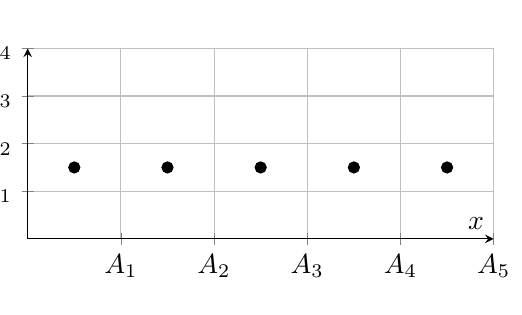
\begin{tikzpicture}[trim axis left, trim axis right]
		\begin{axis}[
		height=4cm,
		width = 7.5cm,
		axis lines=middle,
		xlabel={$x$},
		ylabel={$y$},
		xtick={0,1,2,3,4,5},
		ytick={0,1,2,3,4},
		xticklabels = {0,$A_1$,$A_2$,$A_3$,$A_4$,$A_5$},
		yticklabels = {0,$B_1$,$B_2$,$B_3$,$B_4$},
		ylabel near ticks,
		ymin=0, ymax=4,
		xmin=0, xmax=5,
		grid = both
		]
		\addplot [only marks] table {
		0.5 1.5
		1.5 1.5
		2.5 1.5
		3.5 1.5
		4.5 1.5
		};
		\end{axis}
\end{tikzpicture}
\end{figure}

Vyjádřením $B_j$ můžeme určit \textbf{marginální} pravděpodobnost $P(B_j)$
\begin{eqnarray*}
B_j & = & \bigcup_{i=1}^m B_j\cap A_i\\
P(B_j) & = & P\left(\bigcup_{i=1}^m B_j\cap A_i\right) = \sum_{i=1}^m P(B_j\cap A_i)
\end{eqnarray*}

\subsection{Podmíněná pravděpodobnost}
Podmíněná pravděpodobnost značí pravděpodobnost, že nějaký jev nastane při uvažování hypotézy, že nastal jev jiný (Pravděpodobnost jevu $A$ za podmínky, že vznikl jev $B$). Značí se $P(A|B)$ a nazývá se tzv. \textbf{Bayesův vztah}, který má vzorec

\[ P(A|B) = \frac{P(A\cap B)}{P(B)} \]

\begin{note}{Příklad}
\textbf{Určete, zda jsou následující množiny $\sigma$-algebrami.}

\begin{enumerate}[label=\alph*)]
\item Množina $\omega\in\Omega$ je množinou reálných čísel v intervalu mezi 0 a 1, $\mathscr{U}$ je množina všech podmnožin $\Omega$, které se skládají pouze z racionálních čísel.\br

\textbf{Odpověď:} Nejedná se o $\sigma$-algebru, protože neobsahuje doplňky jevů!

\item Množina $\mathscr{U}$ je množina všech podmnožin $\Omega$, které se skládají pouze z racionálních čísel, ale $\Omega$ je množina všech racionálních čísel mezi 0 a 1.\br

\textbf{Odpověď:} Ano, jedná se o $\sigma$-algebru

\item Množina $\Omega$ je množina všech racionálních čísel mezi 0 a 1. $\mathscr{U}$ je množina všech podmnožin, které jsou konečné nebo mají konečný doplněk.\br
\textbf{Odpověď:} Nejedná se o $\sigma$-algebru, uvnitř množiny $\Omega$ existují nekonečné množiny s nekonečným doplňkem.
\end{enumerate}
\end{note}

\subsection{Náhodná veličina (NV)}
Nechť máme prostor $\{\Omega, \mathscr{U},\mu\}$, (vektorová) náhodná veličina je zobrazením
\[ X:\Omega\to\mathbb{R}^n \]

Pro náhodnou veličinu platí následující podmínky:
\begin{itemize}
\item Elementární jev $\omega\in\Omega$ zobrazuje do nějaké podmnožiny $y\in\mathbb{R}^n$ tak, že každá množina
\[ A=\{\omega, X(\omega)\leq x,x\in\mathbb{R}^n\} \]
je prvek $\sigma$-algebry $\mathscr{U}$.

\item Jsme schopni změřit interval $(-\infty, x)$.
\end{itemize}

\begin{note}{Příklad}
\textbf{Hod mincí}\\
Máme dva nezávislé hody mincí. Množina jevů je $\Omega=\{PP,PO,OP,OO\}$ a sledujeme jev $A_1$, který značí, že \textit{padne alespoň jedna panna}. Pro náhodnou veličinu platí

\[
I_A(\omega) =
\begin{cases}
	1 & \text{pokud } \omega\in A\\
	0 & \text{jinak}
\end{cases}
\]

Potom $X(\Omega)=\{0,1\}$ a \textbf{minimální $\sigma$-algebra} má tvar $\mathscr{U}=\big\{\emptyset, \Omega, OO, \{PO,O,P,PP\}\big\}$. Jevy pak mohou vypadat následovně:
\begin{eqnarray*}
A_1 & = & \{\omega, X(\omega)\leq -1\}=\emptyset\\
A_2 & = & \{\omega, X(\omega)\leq \frac{1}{2}\}="OO"\\
A_3 & = & \{\omega, X(\omega)\leq 5\}=\Omega
\end{eqnarray*}
\end{note}